\documentclass[Lecture.tex]{subfiles}
\begin{document}
\section{Section 3.1-4.1 Review}

\begin{frame}
The scatterplots below display three bivariate data sets.  The correlation coefficients for these data sets are 0.03, 0.68, and 0.89.  Which scatterplot corresponds to the data set with $r=0.03$?
\begin{center}
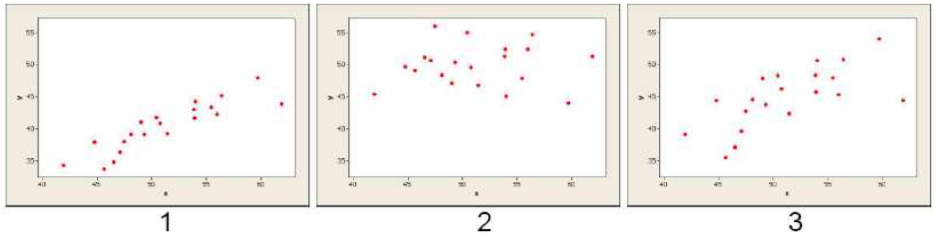
\includegraphics[scale=.3]{scattervote}
\end{center}
{\bf (a)} Plot 1, {\bf (b)} Plot 2, {\bf (c)} Plot 3
\end{frame}

\begin{frame}
Gabriel found a strong correlation in an empirical study showing that individuals' physical ability decreased significantly with age.  Which numerical result below best describes this situation?\\
\begin{center}
{\bf (a)} -1.2\\
{\bf (b)} -1.0\\
{\bf (c)} -0.8\\
{\bf (d)} +0.8\\
{\bf (e)} +1.0
\end{center}
\end{frame}

\begin{frame}
A store manager conducted an experiment in which he systematically varied the width of a display for toothpaste from 3 ft. to 6 ft. and recorded the corresponding number of tubes of toothpaste sold per day.  The data was used to fit a regression line, which was $${\text{tubes sold per day}}=20+10({\text{ display width}})$$
What is the predicted number of tubes sold per day for a display width of 12 feet?\\
{\bf (a)} 120\\
{\bf (b)} 140\\
{\bf (c)} It would be unwise to use the regression line to make a prediction for a display with of 12 feet.
\end{frame}

\begin{frame}
Gas mileage and weight were recorded for each automobile in a sample of 20 compact cars.  There was a strong negative correlation, with $r=-.87$.  Based on the value of $r$, it is reasonable to conclude that increasing the weight of a compact car causes a decrease in gas mileage.\\
{\bf (a)} True, and I am very confident.\\
{\bf (b)} True, and I am not very confident.\\
{\bf (c)} False, and I am not very confident.\\
{\bf (d)} False, and I am very confident.
\end{frame}

\begin{frame}
Which of the following characteristics in a residual plot are indicative of potential problems?\\
{\bf (a)} A strong pattern in the residual plot\\
{\bf (b)} Isolated points in the residual plot\\
{\bf (c)} A lack of any strong pattern in the residual plot\\
{\bf (d)} Both (a) and (b) above are indicative of potential problems.
\end{frame}

\begin{frame}
The following contingency/two-way table classifies the members of a certain government into political party (Liberal or Conservative) and whether they support or oppose the spending bill that is currently up for adoption.
\begin{center}
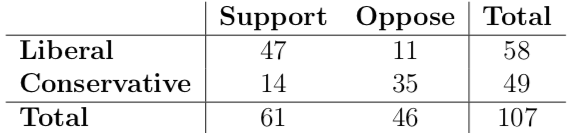
\includegraphics[scale=.4]{contingency}
\end{center}
What fraction of the government members are conservatives who support the bill?\\
{\bf (a)} 14/61, {\bf (b)} 14/49, {\bf (c)} 14/107, {\bf (d)} None of the above.
\end{frame}

\begin{frame}
The following contingency/two-way table classifies the members of a certain government into political party (Liberal or Conservative) and whether they support or oppose the spending bill that is currently up for adoption.
\begin{center}
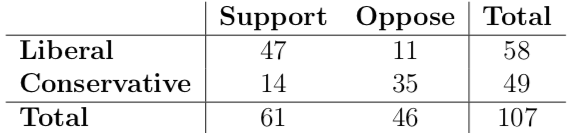
\includegraphics[scale=.4]{contingency}
\end{center}
What fraction of the liberals support the bill?\\
{\bf (a)} 47/61, {\bf (b)} 47/58, {\bf (c)} 47/107, {\bf (d)} None of the above
\end{frame}








\end{document}